\documentclass[a4paper]{article}
\title{Tema Algoritmi Avansati}
\author{Eduard-Valentin Dumitrescul, grupa 232}

\usepackage[legalpaper, portrait, margin=0.8in]{geometry}
\usepackage{lmodern}  % for bold teletype font
\usepackage{amsmath}  % for \hookrightarrow
\usepackage{xcolor}   % for \textcolor
\usepackage{listings}
\lstset{
  basicstyle=\ttfamily,
  mathescape, 
  breaklines=true,
  postbreak=\mbox{\textcolor{blue}{$\hookrightarrow$}\space},
}
\usepackage{hyperref}
\usepackage{graphicx}


\begin{document}
\maketitle
\section{Algoritmi Aproximativi}
\subsection{Knapsack}
Fie S un șir de numere naturale ${s_{1}, s_{2}, ... , s_{n} }$ și K un număr natural, cu $K \geq s_{i}$ pentru orice i între 1 și n.

a) Scrieți un algoritm pseudo-polinomial care găsește suma maximă,
dar care să fie $\leq K$, ce poate fi formată din elementele din S (numere
întregi, pozitive, luate cel mult o singură dată). Indicați complexitatea de timp/spațiu a algoritmului propus de voi și justificați de ce
acesta este corect (de ce soluția găsită este optimă). \hfill(1p)

b) Scrieți un algoritm aproximativ care calculează o sumă cel puțin pe
jumătate de mare ca cea optimă, dar rulează în timp O(n) și complexitate spațiu O(1). \hfill(1p)

\subsubsection*{Rezolvare: a)}


Complexitate: O(N*K) timp si O(K) spatiu
\begin{lstlisting}[tabsize=2]

sum_reached[0] = 1    #suma 0 se obtine in mod implicit
for i=1 to k:
	sum_reached[i] = 0 #marcam faptul ca inca nu am obtinut suma i

#luam, pe rand, fiecare valoare din sirul S si incercam sa obtinem noi sume pe baza celor deja obtinute
for i=1 to n: 
	for sum=k to 0:
		if sum_reached[sum] = 1 and i + sum <= k:
			sum_reached[i+sum] = 1
			
maximum_sum = arg(max(i | i$\in${0,1,...,k}, sum_reached[i] = 1))

\end{lstlisting}

Stim ca suma 0 se poate obtine mereu (nealegand niciun numar din sir).

Presupunem ca am gasit toate sumele $\leq K$ ce pot fi obtinute adunand numere din ${s_{1}, s_{2}, ... , s_{i-1} }$. Acum, orice suma ce il contine pe $s_{i}$ si este formata cu numerele ${s_{1}, s_{2}, ... , s_{i} }$ este de forma $s_{i} + S_{i-1}$ , unde S este o suma obtinuta din numerele ${s_{1}, s_{2}, ... , s_{i-1} }$. Stiind ca am gasit toate astfel de $S_{i-1}$ rezulta ca vom gasi si toate sumele de forma $S_{i}$.
Inductiv, vom gasi toate sumele $S_{n} \leq K$ posibile formate din ${s_{1},s_{2},...,s_{n} }$.



\subsubsection*{Rezolvare: b)}
Complexitate: O(N) timp si O(1) spatiu
\begin{lstlisting}[tabsize=2]

Fie S lista de numere

sum = 0
maxValue = 0
for each s in S:
	if sum + s <= K:
		sum += s
	if max < s:
	 	maxValue = s
	 	
if maxValue >= K/2:
	ALG() = maxValue
else:
	ALG() = sum

\end{lstlisting}

\begin{flushleft}

OPT = valoarea solutiei optime

vmax = valoarea maxima din S

Daca $vmax \geq OPT/2$, atunci $ALG = vmax \geq OPT/2$, deci $ALG \geq 1/2 * OPT$.

Daca $vmax < OPT/2$, atunci fiecare numar din S este $\leq OPT/2$.
Daca algoritmul va insuma toate numerele, atunci obtine solutia optima.
Altfel, fie primul numar $s_{i}$ pe care nu il aduna si $sum$, suma obtinuta pana in acel punct.

$sum + s_{i} > K \geq OPT \Rightarrow sum > OPT - s_{i}$ (1)

$s_{i} < OPT/2 \Rightarrow OPT - s_{i} > OPT/2$ (2)

$(1) si (2) \Rightarrow sum > OPT/2$

$ALG \geq sum \Rightarrow ALG > OPT/2$

Asadar, ALG ete 1/2-aproximativ.

\end{flushleft}

\subsubsection*{Exemplu in care $ALG \approx OPT / 2$:}
\begin{flushleft}

$S = \{10, 1, 2, 3, 4\}, K = 20$ 

$ALG = 10$

$OPT = 20$

$ALG / OPT = 2$
\end{flushleft}


\subsection{Load-Balancing - 2}
Fie $ALG_{1}$ și $ALG_{2}$ doi algoritmi de rezolvare pentru aceeași problemă de minimizare. $ALG_{1}$ este un algoritm 2-aproximativ, respectiv
$ALG_{2}$ este un algoritm 4-aproximativ. Stabiliți valoarea de adevăr a
următoarelor propoziții, dând și o scurtă justificare:


a) Există cu siguranță un input I pentru care
$ALG_{2}(I) \geq 2 \cdot ALG_{1}(I)$ \hfill(0,5p)

b) Nu există niciun input I pentru care
$ALG_{1}(I) \geq 2 \cdot ALG_{2}(I)$ \hfill (0,5p)

\subsubsection*{Rezolvare: a)}
Nu este adevarat. Daca pentru un anume I, amandoi algoritmii dau solutia optima, relatia nu este adevarata.

\subsubsection*{Rezolvare: b)}
\begin{flushleft}
Nu este adevarat.

$ALG_{1}$ este 2-aproximativ $\Rightarrow ALG_{1} \leq 2 \cdot OPT$

Presupunem ca exista I pentru care $ALG_{1} \geq 2 \cdot ALG_{2}$, deci\\
$2 \cdot OPT \geq ALG_{1} \geq 2 \cdot ALG_{2}$, de unde\\
$OPT \geq ALG_{2}$.

Asadar, pentru $ALG_{2} = OPT$ si $ALG_{1}(I) = 2 \cdot OPT(I)$ inegalitatea are loc.
\end{flushleft}

\subsection{Load-Balancing - 3}
Fie algoritmul Ordered-Scheduling Algorithm (cursul 2, slide-ul 42),
care implică algoritmul descris anterior (slide-ul 19) la care adăugăm
o preprocesare cu care sortăm descrescător activitățile după timpul de
desfășurare. Th. 2 afirmă că acest algoritm este $\dfrac{3}{2}-aproximativ$. Arătați
că acest factor de aproximare poate fi îmbunătățit la $\dfrac{3}{2}-\dfrac{1}{2m}$ (unde m
este numărul de calculatoare pe care se pot executa activități). \hfill (2p)

\subsubsection*{Rezolvare}
\begin{flushleft}
Fie $k$ indicele masinii cu loadul maxim in urma executarii algoritmului.

$ALG = load(k)$

Fie $q$ ultima activitate adaugata pe masina $k$

Fie $load'(i)$ load-ul masinii $i$ fix inainte ca activitatea $q$ sa fie asociata masinii $k$.

$ALG = load(K) = load'(k) + t_{q}$

Conform justificarii de la curs:
\begin{center}
$load'(k) + t_{q} \leq \dfrac{1}{m} \sum_{i=1}^{n}t_{i} + t_{q}$
\end{center}

Dar, faptul ca adaugam activitate $q$ la masina $k$ ne spune ca $load`(k)$ este min(load`). Astfel, putem imbunatati inegalitatea:

\begin{center}
$load'(k) + t_{q} \leq \dfrac{1}{m} \sum_{i=1}^{q-1}t_{i} + t_{q}$
\end{center} 

Daca $q \leq m$ atunci $q$ va fi pusa peste o masina goala, deci $ALG = OPT$
Daca $q > m$ atunci:
\begin{center}
$load'(k) + t_{q} \leq \dfrac{1}{m} \sum_{i=1}^{q-1}t_{i} + t_{q} = \dfrac{1}{m} \sum_{i=1}^{q}t_{i} + (1-\dfrac{1}{m})t_{q}$ 

$ \leq \dfrac{1}{m} \sum_{i=1}^{n}t_{i} + (1-\dfrac{1}{m}) \cdot \dfrac{1}{2}(t_{m} + t_{m+1})$

$ \leq OPT + \dfrac{1}{2} OPT  - \dfrac{1}{2m}= (\dfrac{3}{2} - \dfrac{1}{2m})OPT$
\end{center}

\end{flushleft}

\subsection{Traveling Salesman Problem - 2}
Fie $P$ o mulțime de puncte în plan. Din cursurile anterioare știm să
construim un Minimum Spanning Tree pe baza punctelor din $P$. Numim acest arbore $T$. Uneori, adăugând și alte puncte pe lângă cele din
$P$, putem obține un MST cu cost mai mic. Un asemenea arbore, construit prin adăugarea de noduri se numește Steiner Tree. Algoritmii
pentru calcularea de ST-uri sunt de obicei NP-hard.

a) Arătați că există cazuri în care alegând un punct $q \notin P$ obținem un
MST pentru mulțimea de puncte $P\cup\{q\}$ cu un cost mai mic decât
$T$. \hfill (1p)

b) Fie $Q$ o mulțime de puncte în plan, disjunctă față de $P$. Arătați că $T$
este de cel mult două ori mai mare ca și cost față de MST-ul pentru
$P \cup Q$. Altfel spus, odată ce avem un MST pentru $P$, putem îmbunătăți rezultatul adăugând alte puncte, dar niciodată cu mai mult de
un factor de 2. \hfill (2p)

\subsubsection*{Rezolvare: a)}
\begin{flushleft}
Fie $P=\{p_{1}=(0,0), p_{2}(0,2), p_{3}=(2,0), p_{4}=(2,2)\}$ si $q=(1,1)$.

Costul lui $T$ este 
\begin{center}
$dist(p1, p2) + dist(p1, p3) + dist(p2,p4) = 2+2+2 = 6$ 
\end{center}


Costul arborelui partial de cost minim pe baza punctelor $P \cup \{q\}$ este
\begin{center}
$dist(p1,q) + dist(p2,q) + dist(p3,q) + dist(p4,q)=$

$=\sqrt{2} + \sqrt{2} + \sqrt{2} + \sqrt{2}=$

$=4 * sqrt{2} \approx 5.656$
\end{center}

Asadar, acesta este un caz in care alegând un punct $q \notin P$ obținem un
MST pentru mulțimea de puncte $P\cup\{q\}$ cu un cost mai mic decât
$T$.

\end{flushleft}

\subsubsection*{Rezolvare: b)}

\begin{flushleft}
\textbf{Idee:} Pornind de la MST-ul asociat punctelor $P \cup Q$ de cost $C$, construim un arbore partial asociat punctelor $P$ cu costul cel mult $2\cdot C$. Asadar, MST-ul asociat punctelor $P$ va avea cost cel mult dublu, ceea ce trebuie demonstrat.

\textbf{Observatie 1:} Deoarece $P$ si $Q$ sunt multimi de puncte in plan, regula triunghiului este valabila.

Fie $A$ MST-ul asociat punctelor $P \cup Q$, de cost $C$.

Fie $B$ arborele partial asociat punctelor $P$ pe care urmeaza sa-l construim.

\textbf{Observatie 2:} Nu are sens ca un punct $q \in Q$ sa fie frunza in $A$, deoarece, prin eliminarea lui, obtinem un nou MST, de cost mai mic, asociat punctelor $P \cup Q \setminus \{q\}$. Asadar, vom presupune, fara a pierde generalitatea, ca nu exista astfel de puncte.

De asemenea, consideram cu $p \in P$ este radacina arborelui $A$.
\vspace{16pt}

Scriem \href{https://www.infoarena.ro/lowest-common-ancestor}{\underline{parcurgerea Euleriana}} a arborelui $A$.

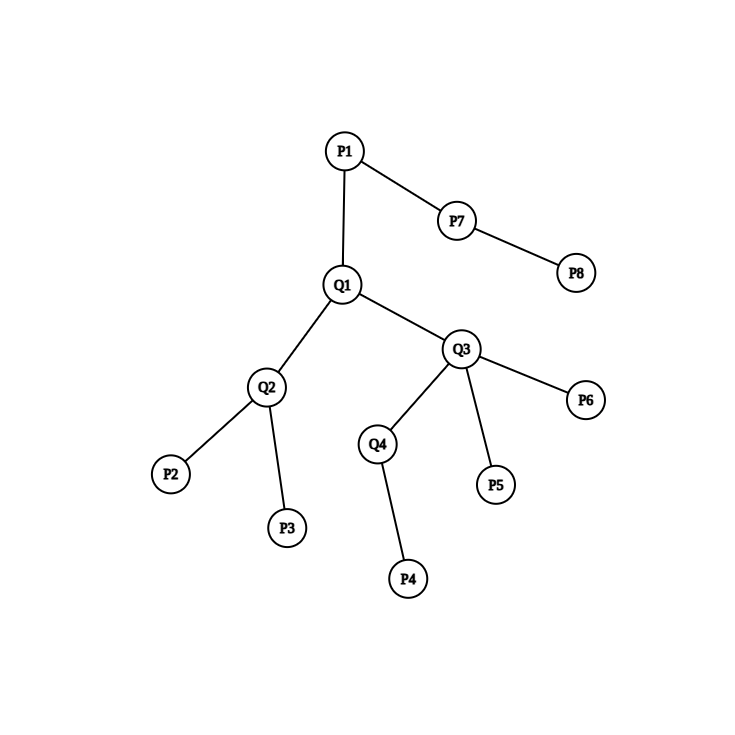
\includegraphics[scale=0.4]{graph.png}

Pentru arborele din imagine, parcurgerea Euleriana este:

P1, Q1, Q2, P2, Q2, P3, Q2, Q1, Q3, Q4, P4, Q4, Q3, P5, Q3, P6, Q3, Q1, P1, P7, P8, P7, P1

Arborele nostru partial $B$ va fi construit in asa fel incat parcurgerea lui Euleriana sa fie identica cu cea a arborelui $A$, dupa ce eliminam punctele din $Q$.

Pentru acest exemplu, parcurgerea Euleriana a arborelui $B$ va fi:
P1 P2 P3 P4 P5 P6 P7 P8 P7 P1

Pentru orice lant (cu eventualele renumerotari) $P1-Q1-Q2-...-Qn-P2$ avem:
\begin{center}
$dist(P1,P2) \leq dist(P1,Q1) + dist(Q1,Q2) + ... + dist(Qn-1, Qn) + dist(Qn, P2)$
\end{center}

Deci, suma distantelor $SB$ dintre toate perechile de puncte consecutive din parcurgerea Euleriana a lui $B$ este mai mica sau egala cu suma dinstantelor $SA$ dintre toate perechile de puncte consecutive din parcurgerea Euleriana a lui $A$.
Cum $SA$ este egal cu lungimea conturului arborelui $A$, avem:
\begin{center}
$SB \leq SA = 2 \cdot C$
\end{center}

Construim graful $G$ in care exista muchie intre Px si Py, daca Px si Py se afla pe pozitii consecutive in parcurgerea Euleriana a lui B. Evident, obtinem chiar arborele $B$.

\begin{center}
$cost MST(B) \leq $ suma costurilor muchiilor lui B $= SB \leq 2 \cdot C$
\end{center}

Asadar, am demonstrat ca, prin adaugarea de noi puncte, putem imbunatati MST-ul lui $P$ cu un facor cel mult 2. 


\end{flushleft}

\end{document}


